% ============================================================================
% ANNEXES
% Structure inspirée du rapport de référence (Amal Rahmeni)
% ============================================================================

\section{Introduction}

Cette annexe regroupe les documents complémentaires et artefacts techniques produits durant le projet Guidni. Elle contient :

\begin{enumerate}
    \item Schéma complet de la base de données
    \item Exemples de conversations avec l'agent
    \item Configuration des modèles LLM
    \item Captures d'écran de l'interface utilisateur
    \item Code source des composants principaux
\end{enumerate}


% ────────────────────────────────────────────────────────────────
\section{Schéma de la base de données}
% ────────────────────────────────────────────────────────────────

\subsection{Entités principales}

Le schéma relationnel complet comprend les tables suivantes :

\begin{itemize}
    \item \textbf{User} : id, email, hashed\_password, created\_at, preferences\_json
    \item \textbf{Conversation} : id, user\_id, title, created\_at, updated\_at
    \item \textbf{Message} : id, conversation\_id, role, content, created\_at
    \item \textbf{Activity} : id, title, description, category, region, city, price, duration, opening\_hours
    \item \textbf{Stay} : id, name, description, category, region, city, price, amenities
    \item \textbf{Restaurant} : id, name, description, cuisine\_type, region, city, price\_range
    \item \textbf{Attraction} : id, name, description, category, latitude, longitude
    \item \textbf{Rental} : id, vehicle\_type, provider, price\_per\_day
    \item \textbf{Transfer} : id, from\_location, to\_location, vehicle\_type, price
    \item \textbf{LinUCBGlobal} : matrix\_a (306x306), vector\_b (306), updated\_at
    \item \textbf{UserProfile} : user\_id, context\_vector (9), decay\_factor, last\_updated
    \item \textbf{BehavioralEvent} : id, user\_id, item\_id, event\_type, reward\_value, timestamp
\end{itemize}

\begin{figure}[H]
    \centering
    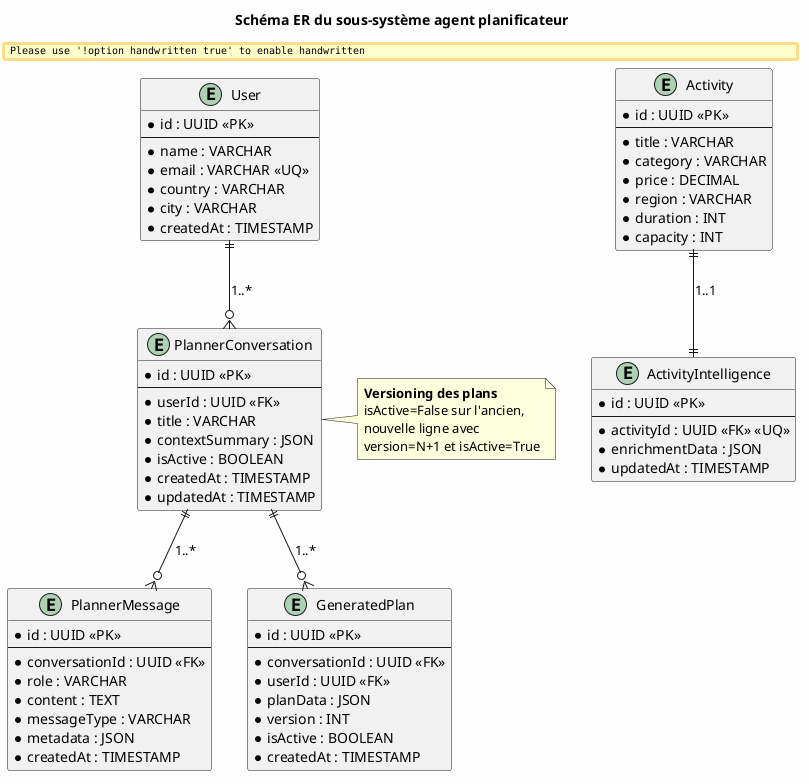
\includegraphics[width=\textwidth]{diagrams/fig_03_er_diagram_planner.png}
    \caption{Diagramme entité-relation — Partie Planificateur}
    \label{fig:er_planner}
\end{figure}

\begin{figure}[H]
    \centering
    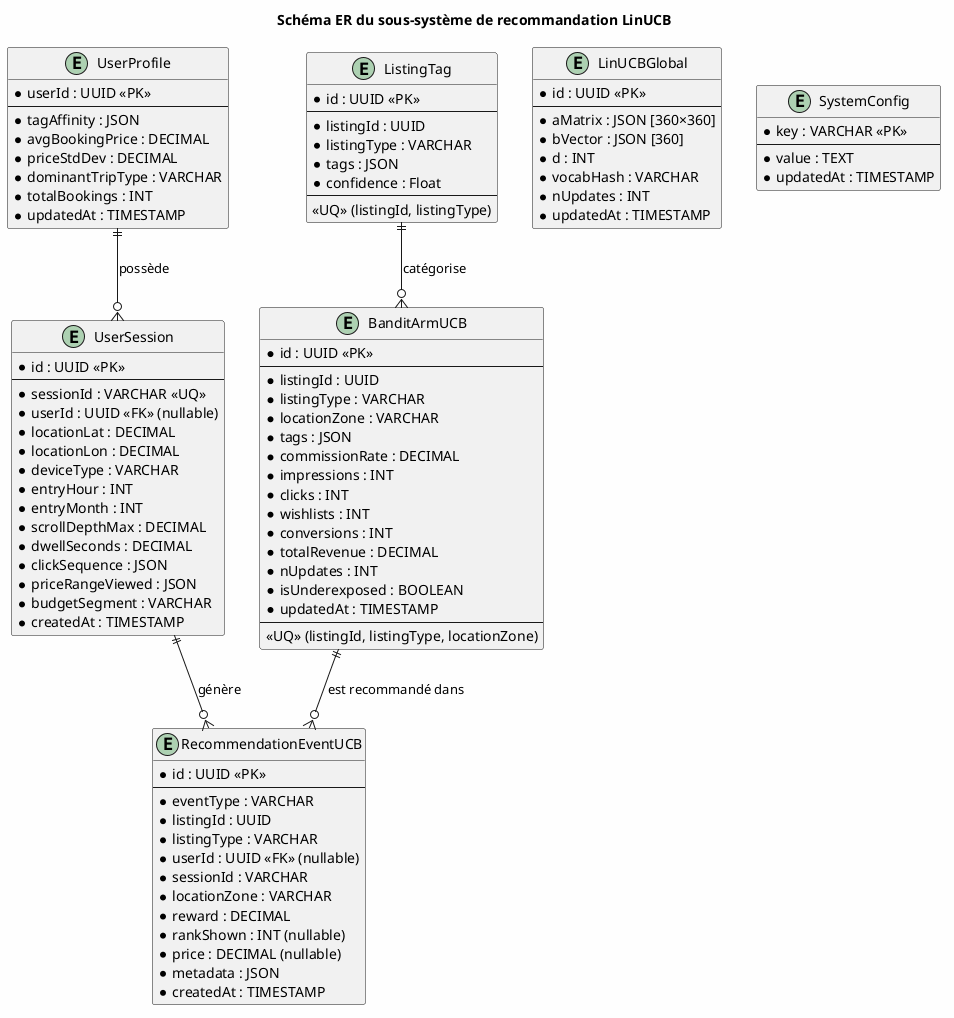
\includegraphics[width=\textwidth]{diagrams/fig_03_er_diagram_recommender.png}
    \caption{Diagramme entité-relation — Partie Recommandation}
    \label{fig:er_recommender}
\end{figure}


% ────────────────────────────────────────────────────────────────
\section{Exemples de conversations}
% ────────────────────────────────────────────────────────────────

\subsection{Requête en français}

\begin{lstlisting}[language=Python, caption=Exemple de requête utilisateur]
{
  "user_id": "usr_12345",
  "message": "Je veux un plan de 3 jours à Djerba pour une famille avec 2 enfants, budget 400 TND par jour"
}
\end{lstlisting}

\subsection{Réponse de l'agent}

\begin{lstlisting}[language=Python, caption=Exemple de réponse structurée]
{
  "plan": {
    "day_1": [
      {"time": "09:00", "activity": "Plage de Sidi Mahrez", "type": "beach"},
      {"time": "13:00", "activity": "Restaurant Le Golfe", "type": "lunch"},
      {"time": "15:00", "activity": "Visite de Houmt Souk", "type": "culture"}
    ],
    ...
  },
  "total_budget": "1200 TND",
  "recommendations": [...]
}
\end{lstlisting}


% ────────────────────────────────────────────────────────────────
\section{Configuration des modèles LLM}
% ────────────────────────────────────────────────────────────────

\begin{table}[H]
    \centering
    \caption{Configuration des fournisseurs LLM}
    \label{tab:llm_config}
    \small
    \begin{tabular}{p{2cm} p{3cm} p{3cm} p{4cm}}
        \toprule
        \textbf{Fournisseur} & \textbf{Modèle} & \textbf{Température} & \textbf{Usage} \\
        \midrule
        Ollama & qwen2.5:7b & 0.7 & Développement local \\
        Groq & llama-3.3-70b & 0.5 & Production rapide \\
        Gemini & gemini-2.5-flash & 0.6 & Requêtes complexes \\
        Lightning & gpt-5 & 0.7 & Fallback premium \\
        \bottomrule
    \end{tabular}
\end{table}


% ────────────────────────────────────────────────────────────────
\section{Captures d'écran}
% ────────────────────────────────────────────────────────────────

\begin{figure}[H]
    \centering
    
\includegraphics[width=0.8\textwidth]{diagrams/screen_A4_chat_interface.png}
    \caption{Interface de chat Guidni}
    \label{fig:screen_chat}
\end{figure}

\begin{figure}[H]
    \centering
    
\includegraphics[width=0.8\textwidth]{diagrams/screen_04_chat_plan_output.png}
    \caption{Sortie de plan de voyage}
    \label{fig:screen_plan}
\end{figure}

\begin{figure}[H]
    \centering
    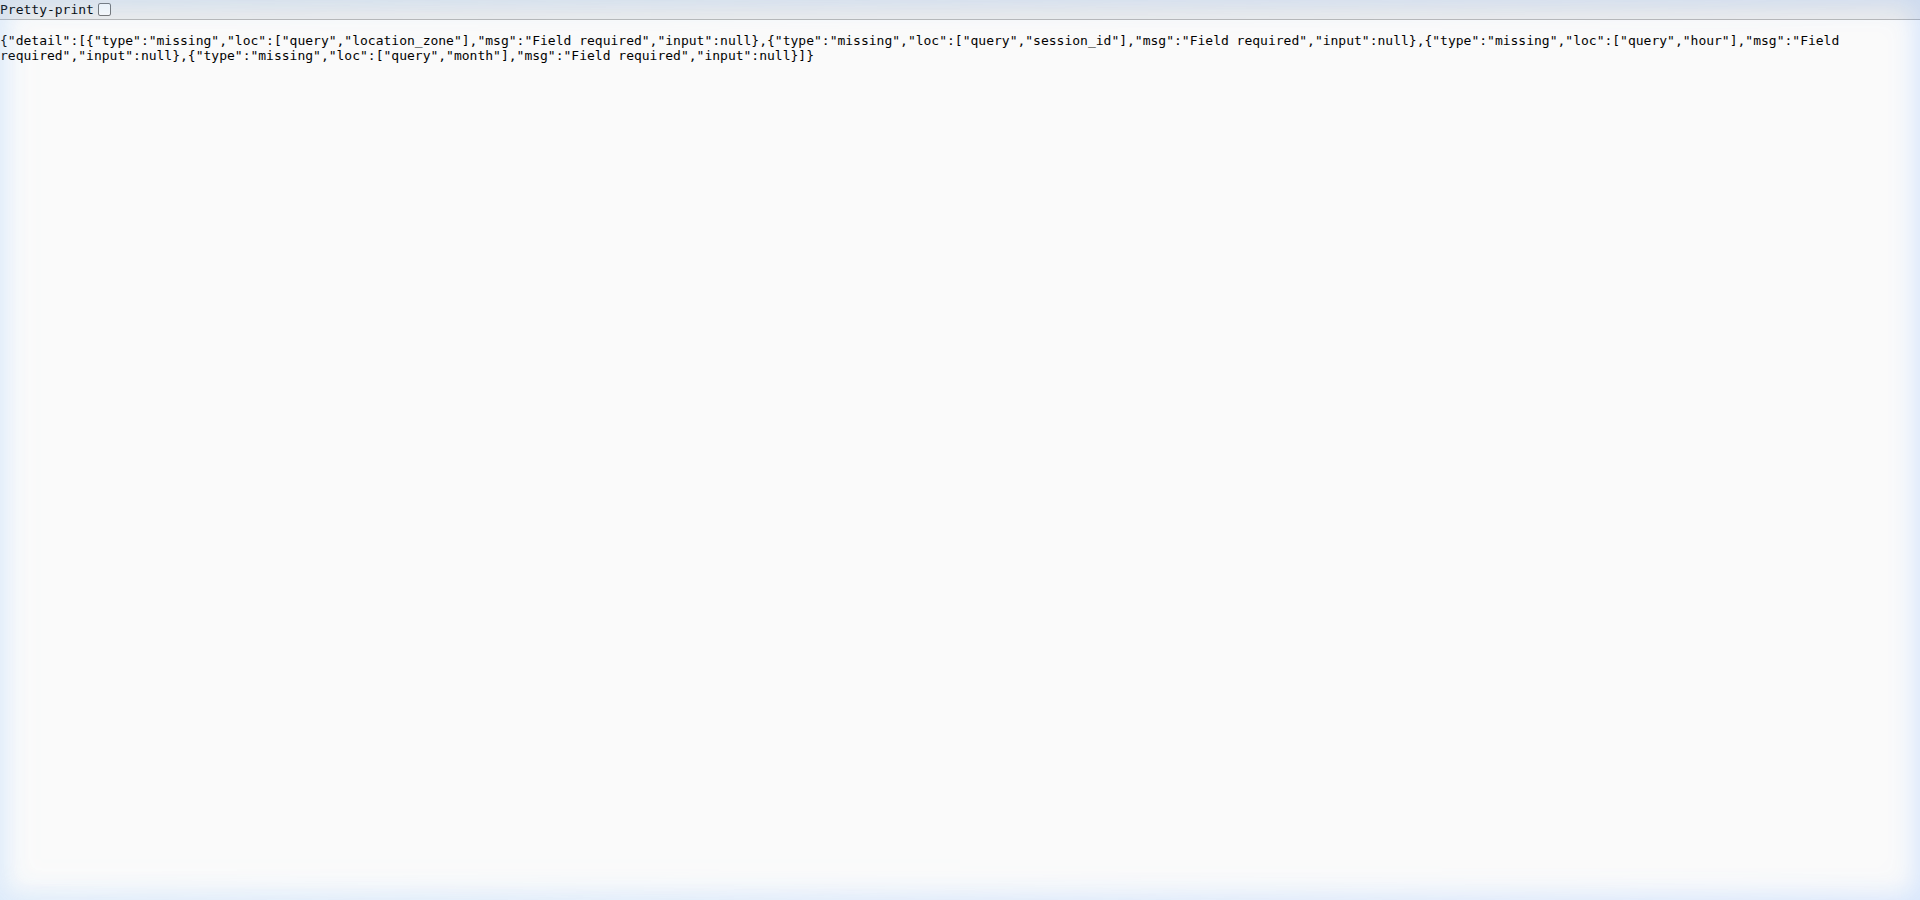
\includegraphics[width=0.8\textwidth]{diagrams/screen_A4_recommendations_response.png}
    \caption{Réponse avec recommandations LinUCB}
    \label{fig:screen_recommendations}
\end{figure}

\begin{figure}[H]
    \centering
    
\includegraphics[width=0.8\textwidth]{diagrams/screen_A4_admin_rebuild.png}
    \caption{Endpoint admin de reconstruction RAG}
    \label{fig:screen_admin}
\end{figure}


% ────────────────────────────────────────────────────────────────
\section{Code source des composants clés}
% ────────────────────────────────────────────────────────────────

\subsection{Agent State LangGraph}

\begin{lstlisting}[language=Python, caption=Définition de AgentState]
class AgentState(TypedDict):
    messages: Annotated[list[AnyMessage], operator.add]
    profile: dict
    activities: list
    stays: list
    restaurants: list
    weather: dict
    locations: list
    rag_context: str
    plan_structure: dict
    thinking_steps: list
    tools_used: list
    iteration_count: int
    needs_more_info: bool
    is_plan_ready: bool
\end{lstlisting}

\subsection{Scoring LinUCB}

\begin{lstlisting}[language=Python, caption=Fonction de scoring LinUCB]
def compute_score(phi: np.ndarray, A: np.ndarray, b: np.ndarray, alpha: float) -> float:
    A_inv = np.linalg.inv(A)
    theta = A_inv @ b
    mean = phi @ theta
    uncertainty = alpha * np.sqrt(phi @ A_inv @ phi)
    return mean + uncertainty
\end{lstlisting}


% ────────────────────────────────────────────────────────────────
\section{Glossaire des abréviations}
% ────────────────────────────────────────────────────────────────

\begin{table}[H]
    \centering
    \caption{Liste des abréviations}
    \label{tab:abbreviations}
    \small
    \begin{tabular}{p{2cm} p{10cm}}
        \toprule
        \textbf{Abréviation} & \textbf{Signification} \\
        \midrule
        API & Application Programming Interface \\
        ASGI & Asynchronous Server Gateway Interface \\
        ERM & Entity-Relationship Model \\
        IA & Intelligence Artificielle \\
        JWT & JSON Web Token \\
        LLM & Large Language Model \\
        NLP & Natural Language Processing \\
        ORM & Object-Relational Mapping \\
        PO & Product Owner \\
        RAG & Retrieval-Augmented Generation \\
        RLHF & Reinforcement Learning from Human Feedback \\
        SM & Scrum Master \\
        SSR & Server-Side Rendering \\
        UCB & Upper Confidence Bound \\
        UNESO & United Nations Educational, Scientific and Cultural Organization \\
        US & User Story \\
        \bottomrule
    \end{tabular}
\end{table}
